\documentclass[10pt, aspectratio=169]{beamer}

% Theme Choice
\usetheme{metropolis} 
\usecolortheme{owl} % Professional dark theme, very eye-soothing

\usepackage[utf8]{inputenc}
\usepackage{amsmath, amssymb, amsthm}
\usepackage{tikz}
\usetikzlibrary{graphs, graphs.standard, positioning, shapes.geometric}

% Title Page Info
\title{The Complexity of Graph Isomorphism}
\subtitle{A Journey from NP-Intermediate to Quasi-Polynomial Time}
\author{Your Name}
\date{\today}
\institute{Department of Computer Science}

\begin{document}

% 1. Title Slide
\maketitle

% 2. Overview
\begin{frame}{Roadmap}
    \tableofcontents
\end{frame}

\section{Introduction: The Visual Puzzle}

% 3. What is GI?
\begin{frame}{What is Graph Isomorphism (GI)?}
    \begin{itemize}
        \item \textbf{Core Question:} Are these two graphs structurally identical?
        \item \textbf{The Catch:} They are drawn differently and labeled differently.
    \end{itemize}
    \begin{center}
        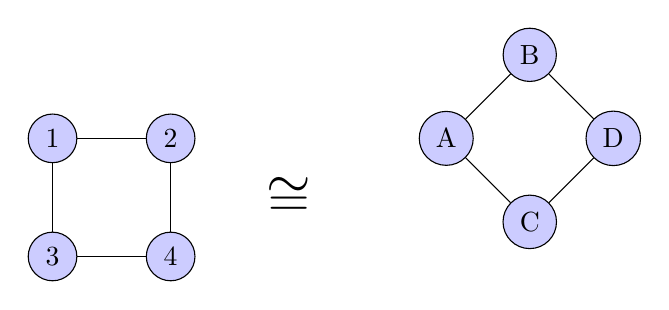
\begin{tikzpicture}[nodes={draw, circle, fill=blue!20}, node distance=1.5cm]
            % Graph G
            \node (n1) {1};
            \node (n2) [right of=n1] {2};
            \node (n3) [below of=n1] {3};
            \node (n4) [right of=n3] {4};
            \draw (n1) -- (n2) -- (n4) -- (n3) -- (n1);
            
            \node[draw=none, fill=none] at (3, -0.75) {\huge $\cong$};
            
            % Graph H (Drawn as a diamond)
            \begin{scope}[xshift=5cm]
                \node (ma) {A};
                \node (mb) [above right of=ma] {B};
                \node (mc) [below right of=ma] {C};
                \node (md) [below right of=mb] {D};
                \draw (ma) -- (mb) -- (md) -- (mc) -- (ma);
            \end{scope}
        \end{tikzpicture}
    \end{center}
\end{frame}

% 4. Formal Definition
\begin{frame}{Formal Definition}
    Two graphs $G=(V_G, E_G)$ and $H=(V_H, E_H)$ are isomorphic if there exists a bijection $f: V_G \to V_H$ such that:
    \[ (u, v) \in E_G \iff (f(u), f(v)) \in E_H \]
    
    \vspace{0.5cm}
    \textbf{The Challenge:}
    \begin{itemize}
        \item There are $n!$ possible bijections (mappings).
        \item For $n=100$, $n!$ is larger than the number of atoms in the universe.
    \end{itemize}
\end{frame}

\section{The Complexity Mystery}

% 5. Complexity Classes
\begin{frame}{Where does it live?}
    \begin{itemize}
        \item \textbf{P:} Polynomial time (Easy).
        \item \textbf{NP-Complete:} Hard (e.g., SAT, Traveling Salesperson).
        \item \textbf{GI-Complete:} Its own category!
    \end{itemize}
    \pause
    \begin{block}{The "Limbo" Problem}
        GI is one of the few problems in \textbf{NP} not known to be in \textbf{P} or \textbf{NP-Complete}. It is often called an \textit{NP-Intermediate} candidate.
    \end{block}
\end{frame}

% 6. Why not NP-Complete?
\begin{frame}{Why it's likely NOT NP-Complete}
    \textbf{Schöning's Theorem (1988):}
    If GI were NP-Complete, then the \textbf{Polynomial Hierarchy (PH)} would collapse to the second level.
    
    \vspace{0.5cm}
    \begin{itemize}
        \item Most researchers believe $PH$ does not collapse.
        \item Therefore, GI must be "easier" than NP-Complete problems.
    \end{itemize}
\end{frame}

\section{The 2015 Breakthrough}

% 7. László Babai
\begin{frame}{The Babai Breakthrough (2015)}
    \begin{itemize}
        \item \textbf{Who:} László Babai (University of Chicago).
        \item \textbf{What:} An algorithm running in \textbf{Quasi-Polynomial Time}.
    \end{itemize}
    
    \[ 2^{O((\log n)^c)} \]
    
    \begin{itemize}
        \item Much faster than exponential $2^n$.
        \item Just a step away from true Polynomial time $n^k$.
    \end{itemize}
\end{frame}

\section{Solving in Practice: The WL-Test}

% 8. Color Refinement Animation
\begin{frame}{The Weisfeiler-Lehman (WL) Test}
    A "Color Refinement" heuristic used in the real world.
    
    \textbf{Step 1: Initialization}
    \begin{itemize}
        \item Label every node with its degree (e.g., all nodes with 3 neighbors get color "Blue").
    \end{itemize}
    \pause
    \textbf{Step 2: Refinement (The Animation)}
    \begin{itemize}
        \item Each node gets a new color based on the multiset of its neighbors' colors.
        \item \textit{Iterate} until colors stabilize.
    \end{itemize}
\end{frame}

% 9. Real World Applications
\begin{frame}{Real World Applications}
    \begin{columns}
        \column{0.5\textwidth}
        \textbf{Chemoinformatics}
        \begin{itemize}
            \item Comparing molecular structures.
        \end{itemize}
        \vspace{0.5cm}
        \textbf{Circuit Verification}
        \begin{itemize}
            \item Matching physical chips to digital designs.
        \end{itemize}
        
        \column{0.5\textwidth}
        \textbf{Code Fingerprinting}
        \begin{itemize}
            \item Detecting software plagiarism.
        \end{itemize}
    \end{columns}
\end{frame}

% 10. Conclusion
\begin{frame}{Summary}
    \begin{itemize}
        \item GI is a unique "Limbo" problem in Complexity Theory.
        \item Too much math structure to be NP-Complete; too hard to be (proven) P.
        \item Babai's result brought us to the doorstep of Polynomial time.
        \item \textbf{Future:} Will someone finally prove $GI \in P$?
    \end{itemize}
\end{frame}

\end{document}